
\section{Qualitative Evaluation}\label{sec:qual}

For the qualitative evaluation, 3 of the paper's authors independently rated 100 randomly-selected image reconstructions from each of the three nearest neighbor methods described in sec. \ref{sec:nn}: \emph{naive}, \emph{pca}, and \emph{pca+u} (all 3 raters received the same set of images). The following rating scheme was used:

\begin{table}
\begin{tabular}{| l | l|}
 \hline
\textbf{ranking} & \textbf{requirement}  \\ \hline
5 & no visible distortions \\ \hline
4 & only minor distortions \\ \hline
3 & distortions present, but objects are recognizable  \\ \hline
2 & pretty large distortions, but scene is recognizable  \\ \hline
1 & severe distortions, scene is not recognizable  \\ \hline
\end{tabular}
\caption{The quality evaluation scheme used.}
\label{tb:rankings}
\end{table}

None of the raters received any instructions other than the rating scheme, and the evaluation was not further discussed. Nevertheless, all the raters were highly correlated with each other, where the inter-rater correlation ranged from 0.71 to 0.75 on the \emph{naive} images, 0.51 to 0.61 on the \emph{pca} images, and 0.59 to 0.64 on the \emph{pca+u} images. In figure \ref{fig:qual_method}a we plot the mean and standard error image rating for each rater and each NN method. We see some differences between the raters, but most notably, the \emph{pca} approach was rated highest across all 3 raters, and when taking the average ratings (over all 3 raters), the reconstruction quality is statistically significantly better rated for the \emph{pca} method over the \emph{naive} method. 

Next, to determine whether ratings corresponded to the actual compression ratio for the images, we correlated each of the rater's scores with the image compression ratios, and then considered different combinations of the rater scores (min, max, mean, mode, median) to see which statistic over the subjective ratings might be most predictive of the objective image compression (see table \ref{tab:corr}). Because raters are highly subjective as to what they consider a reasonable reconstruction (even given the criteria above), we will use the mean rating across all raters as it is most correlated with image compression, and most consistent. In figure \ref{fig:recon} we demonstrate the \emph{pca} NN method reconstructions of a set of images with large compression ratios, that also received high quality ratings (taking the mean across raters). This figure gives a little more insight about how our system works, because naturally, the images with the highest ratings are going to be the ones that benefit least from compression, and that is a less interesting case to consider. We are interested in reasonable reconstructions with great cost savings. We plot the trade-off between compression ratio and reconstruction quality in fig. \ref{fig:qual_method}b. As expected, quality ratings go down as the compression ratio increases. Depending on the application, the optimal point can be chosen.

\begin{table*}
\centering
\begin{tabular}{|c|c|c|c|c|c|c|c|c|}
 \hline
\textbf{method} & \textbf{rater 1} & \textbf{rater 2} & \textbf{rater 3}  & \textbf{min} & \textbf{max} & \textbf{mean} & \textbf{mode} & \textbf{median}\\ \hline
naive & 0.7337 & 0.6700 & 0.6203  & 0.7247 & 0.6837 & \textbf{0.7484} & 0.6324 & 0.6636 \\ \hline
pca & 0.7450 & 0.7916 & 0.5061 & 0.6999 & 0.6791 &  \textbf{0.8070} & 0.6695 & 0.7349 \\ \hline
pca+u & 0.6169 & 0.6685 & 0.6934 & 0.6340 & 0.6755 &  \textbf{0.7635} & 0.6043 & 0.7276  \\ \hline
\end{tabular}
\caption{Here we determine what function of rater scores is most predictive of image compression ratios. We see that the mean across the rater scores has the highest correlation with image compression, presumably because it filters out the noise inherent in subjective judgements.}
\label{tab:corr}
\end{table*}

 \begin{figure*}
%\hspace{-5mm}
%\centering
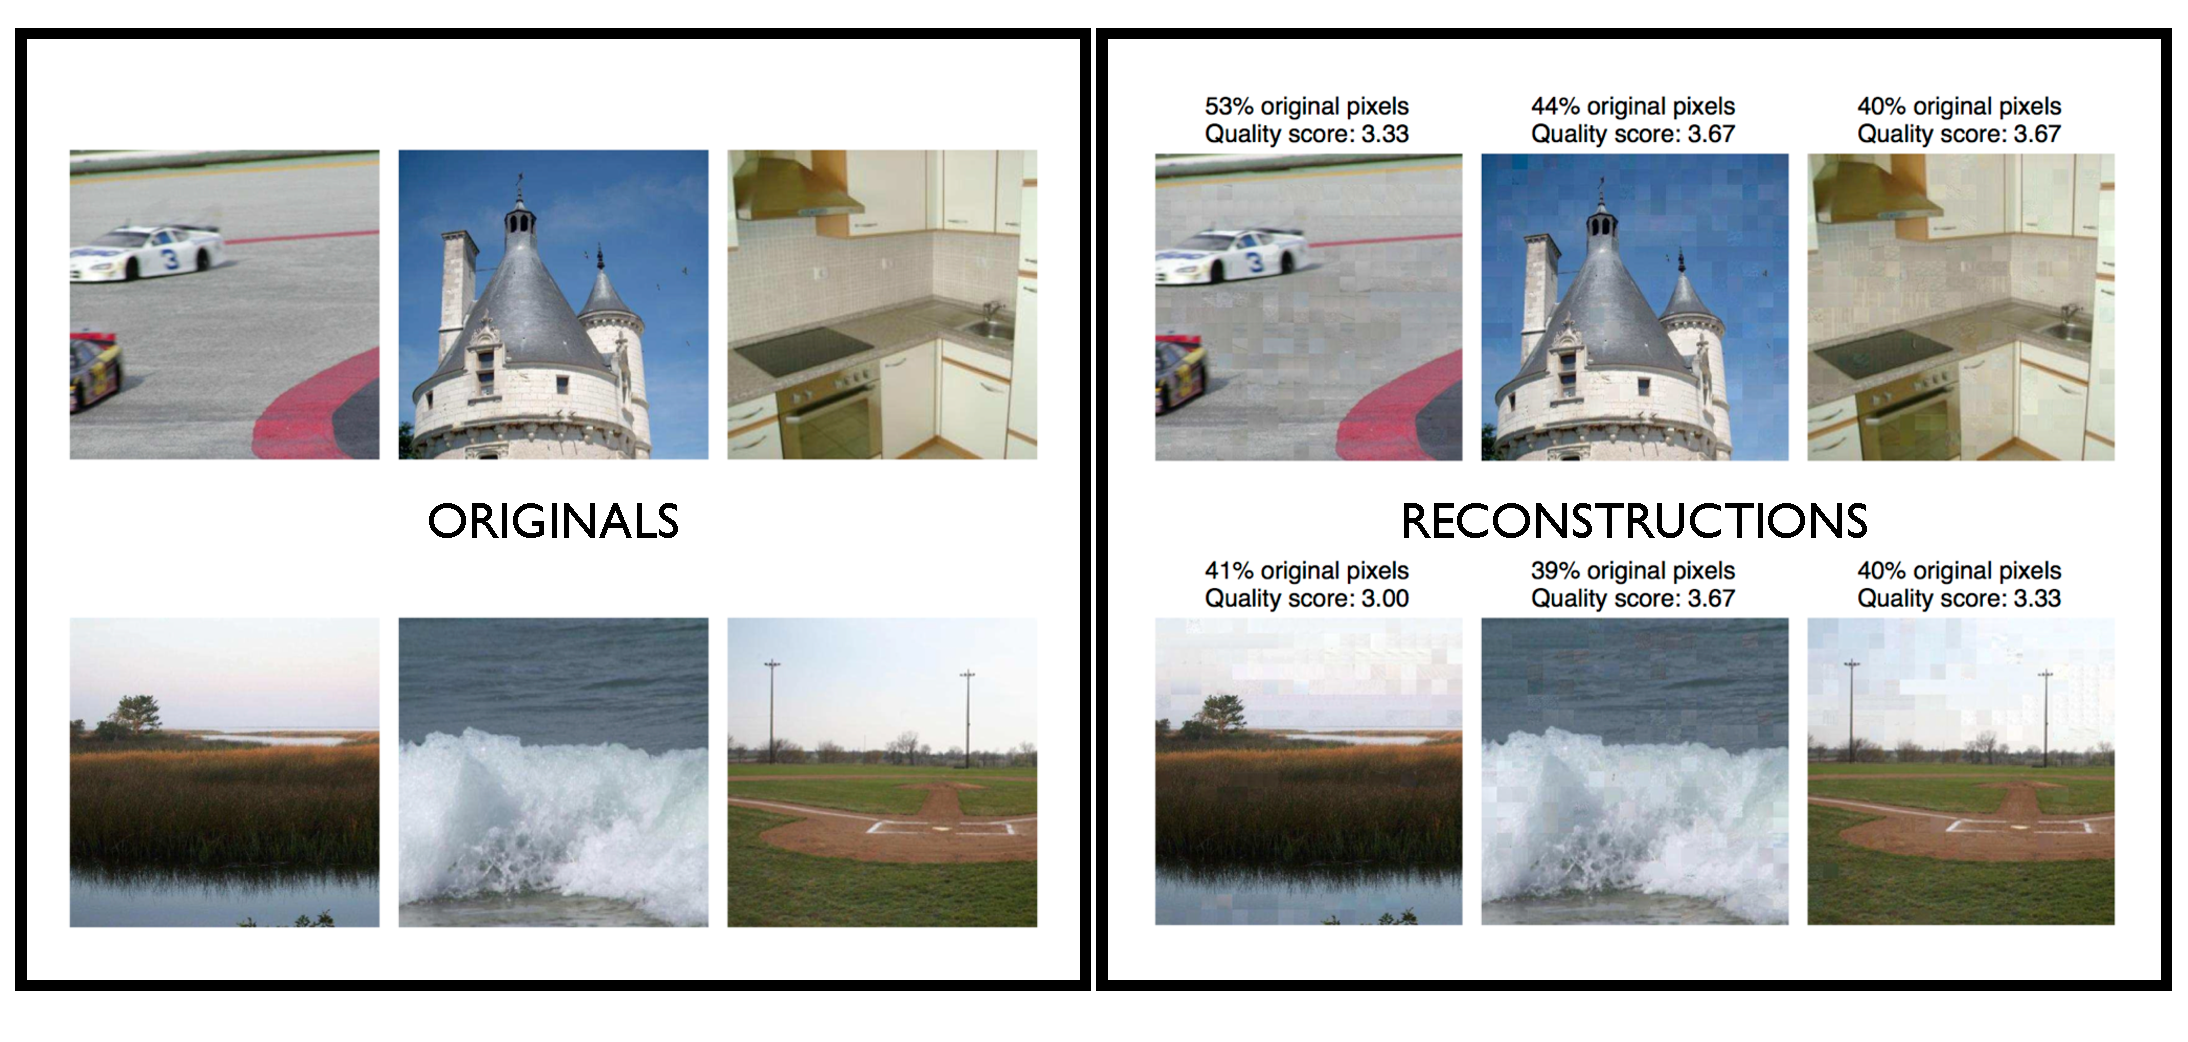
\includegraphics[width=1\linewidth]{fig_quality/orig_recon.pdf}
\caption{Here we plot 6 sample reconstructions (using the \emph{pca} NN method) that had high compression ratios \emph{and} relatively high ratings (mean over 3 raters). }
\label{fig:recon}
\end{figure*}

 \begin{figure*}
%\hspace{-5mm}
\centering
(a)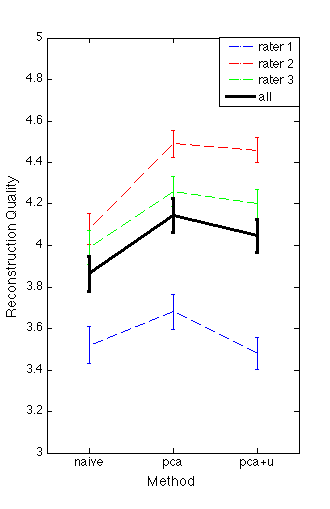
\includegraphics[width=0.3\linewidth]{fig_quality/quality_by_method.png}
(b)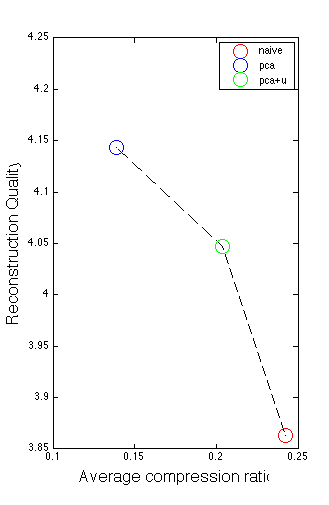
\includegraphics[width=0.3\linewidth]{fig_quality/qual_compr.png}
\caption{(a) Although there is some difference across ratings, all raters agree that the \emph{pca} NN method produces the highest quality reconstructions. (b) Reconstruction quality is inversely proportional to compression ratio. Different applications might desire different settings.}
\label{fig:qual_method}
\end{figure*}
